\documentclass{ltjsarticle}

\usepackage{listings, xcolor}
\usepackage{graphicx}

\lstset{
    basicstyle = {\ttfamily}, % 基本的なフォントスタイル
    frame = {tbrl}, % 枠線の枠線。t: top, b: bottom, r: right, l: left
    breaklines = true, % 長い行の改行
    numbers = left, % 行番号の表示。left, right, none
    showspaces = false, % スペースの表示
    showstringspaces = false, % 文字列中のスペースの表示
    showtabs = false, % タブの表示
    keywordstyle = \color{blue}, % キーワードのスタイル。intやwhileなど
    commentstyle = {\color[HTML]{1AB91A}}, % コメントのスタイル
    identifierstyle = \color{black}, % 識別子のスタイル 関数名や変数名
    stringstyle = \color{brown}, % 文字列のスタイル
    captionpos = b % キャプションの位置 t: 上、b: 下
    literate={_}{\_}1 % アンダースコアのエスケープ
}
\renewcommand{\lstlistingname}{プログラム}

\begin{document}

\title{データ構造とアルゴリズム実験レポート\\
課題:2分木、2分探索木}
\author{202110796 4クラス 高橋大粋}
\date{締切日:2024年11月18日\\
\today}
\maketitle

\section{基本課題}
この課題では、教科書リスト2.11から2.12(p.40から41)の二分木のCプログラムbinarytree.cと、
教科書リスト4.3から4.7(p.69から77)の二分探索木のCプログラムbinarysearchtree.cのリストお
よび実行結果を示した。
\subsection{2分木の実装}\label{subsec:2分木の実装}
\subsubsection{実装の方針}\label{subsubsec:実装の方針1}
まず、二分木の機能としてlabelを節点のラベル、左部分木の根をleft、右部分木の根をrightとする二分木を
作成し、作成した節点のポインタを返すcreate\_node()、節点nを根とする二分木を探索し、行きがけ順で
節点のラベルを標準出力に表示するpreorder()、節点nを根とする二分木を探索し、通りがけ順で節点の
ラベルを標準出力に表示するinorder()、節点nを根とする二分木を探索し、帰りがけ順で節点のラベルを標準出力に
表示するpostorder()、節点nを根とする二分木を幅優先探索し、節点のラベルを標準出力に表示する
breadth\_first\_search()、節点nを根とする二分木の構造が完全にわかる形式で標準出力に表示するdisplay()、
節点nを根とする二分木の高さを返すheight()、節点nを根とする二分木を削除するdelete\_tree()
をbinarytree.cに実装した。また、main関数は別ファイルmain\_binarytree.cに実装した。
\subsubsection{実装コードおよびコードの説明}\label{subsubsec:実装コードおよびコードの説明1}
プログラム\ref{code:one}に、binarytree.cの主要部を示す。 \\ \indent
Node *create\_node(char *label,Node *left,Node *right)関数は、節点とラベルのメモリを確保し、label、
left、rightそれぞれに節点のラベル、左部分木の根、右部分木の根を割り当て初期化し、節点のポインタを返す。
void preorder(Node *n)関数は、方式識別のための文字列PRE:を表示するためにstatic int is\_first\_callを用いて
関数が最初に呼び出されたときだけPRE: を表示する。また、この関数では再帰を用いて行きがけ順での木の走査を
実装しているが、再帰の終了後に改行するためにrootに根を記憶しておき、初回呼び出しでなく引数が根のときに
再帰が終了したとみなし、改行する。
void inorder(Node *n)関数は、preorderと同様に初回呼び出しでIN: を表示し、通りがけ順で木の走査をし、
再帰終了後に改行する。
void postorder(Node *n)関数は、preorderと同様に初回呼び出しでPOST: を表示し、帰りがけ順で木の走査をし、
再帰終了後に改行する。
void display(Node *n)関数は、preorderと同様に初回呼び出しでTREE: を表示し、ノードがNULLならnullを、
ノードにラベルがあるならlabel(を表示する。この関数でも再帰を用いており、左の子に移動した後に,を、右の子に
移動した後に)を表示することにより、X(L,R)という形式で二分木の構造が完全にわかるように表示できる。ここでXはラベル
Lは左部分木、Rは右部分木を表す。また、再帰終了後に改行する。
void breadth\_first\_search(Node *n)関数は、課題2で実装したキューをNode型を扱えるように改良して利用している。
サイズが100のキューを作成し、ルートノードをキューに追加し、BFS: を表示する。キューがからになるまで次を繰り返す。キューの先頭からノードを
取り出す、そのノードのラベルを出力、左の子ノードが存在すればキューに追加、右の子ノードが存在すればキューに追加。
探索が終了したら改行し、キューを開放する。
int height(Node *n)関数は、節点nがNULLなら高さ0を返し、根のみの場合は高さ1を返す。
左部分木と右部分木それぞれで再帰を用いて高さを計算し、大きい方の値+1を高さとして返す。
void delete\_tree(Node *n)関数は、再帰を用いて節点nとその子が確保したメモリをすべて開放する。また、
ラベルが確保したメモリも開放する。\\
なお、これらの関数では節点がNULLの場合は基本的に何もせず終了する。

\begin{lstlisting}[caption=binarytree.cの主要部, label=code:one, language=C, captionpos = b]
Node *create_node(char *label, Node *left, Node *right){
    Node *node = (Node *)malloc(sizeof(Node));
    if (node == NULL) {
        fprintf(stderr, "メモリの割り当てに失敗しました\n");
        exit(EXIT_FAILURE);
    }
     node->label = (char *)malloc(strlen(label) + 1);
    if (node->label == NULL) {
        fprintf(stderr, "文字列用のメモリ割り当てに失敗しました\n");
        free(node);
        exit(EXIT_FAILURE);
    }
    strcpy(node->label, label);
    node->left = left;
    node->right = right;
    return node;
}

void preorder(Node *n){
    static int is_first_call = 1;
    static Node *root = NULL;

    if (is_first_call) {
        printf("PRE: ");
        is_first_call = 0;
        root = n;
    }
    if (n == NULL) return;
    printf("%s ", n->label);
    preorder(n->left);
    preorder(n->right);
    if(is_first_call == 0 && n == root) {
        printf("\n");
    }
}

void inorder(Node *n){
    static int is_first_call = 1;
    static Node *root = NULL;

    if(is_first_call){
        printf("IN: ");
        is_first_call = 0;
        root = n;
    }
    if (n == NULL) return;
    inorder(n->left);
    printf("%s ", n->label);
    inorder(n->right);
    if (is_first_call == 0 && n == root) {
        printf("\n");
    }
}

void postorder(Node *n){
    static int is_first_call = 1;
    static Node *root = NULL;

    if (is_first_call) {
        printf("POST: ");
        root = n;
        is_first_call = 0;
    }
    if (n == NULL) return;
    postorder(n->left);
    postorder(n->right);
    printf("%s ", n->label);
    if (is_first_call == 0 && n == root) {
        printf("\n");
    }
}

void display(Node *n){
    static int is_first_call = 1;
    static Node *root = NULL;

    if (is_first_call) {
        printf("TREE: ");
        root = n;
        is_first_call = 0;
    }

    if (n == NULL) {
        printf("null");
        return;
    }

    printf("%s(", n->label);
    display(n->left);
    printf(",");
    display(n->right);
    printf(")");

    if (is_first_call == 0 && n == root) {
        printf("\n");
        is_first_call = 1;
    }
}

void breadth_first_search(Node *n){
    if (n == NULL) return;

    Queue *q = create_queue(100); 
    enqueue(q, n);

    printf("BFS: ");
    while (q->front != q->rear) { 
        Node *current = dequeue(q);
        printf("%s ", current->label);

        if (current->left != NULL) enqueue(q, current->left);
        if (current->right != NULL) enqueue(q, current->right);
    }
    printf("\n");
    delete_queue(q); 
}

int height(Node *n){
    if (n == NULL) return 0;
    int left_height = height(n->left);
    int right_height = height(n->right);
    return 1 + (left_height > right_height ? left_height : right_height);
}

void delete_tree(Node *n){
    if (n == NULL) return;
    delete_tree(n->left);
    delete_tree(n->right);
    free(n->label);
    free(n);
}
\end{lstlisting}
\subsubsection{実行結果}\label{subsubsec:実行結果1}
まず、main\_binarytree.cを以下に示す。
\begin{lstlisting}
  int main(void) {
    // Build a binary tree
    Node *i = create_node("I", NULL, NULL);
    Node *h = create_node("H", NULL, NULL);
    Node *g = create_node("G", NULL, NULL);
    Node *d = create_node("D", NULL, NULL);
    Node *e = create_node("E", NULL, i);
    Node *f = create_node("F", h, g);
    Node *c = create_node("C", d, e);
    Node *b = create_node("B", f, NULL);
    Node *a = create_node("A", c, b);

    preorder(a);
    inorder(a);
    postorder(a);
    breadth_first_search(a);
    display(a);

    printf("height: %d\n", height(a));

    delete_tree(a);

    return EXIT_SUCCESS;
}
\end{lstlisting}
今回は次の図で表す二分木に対して、実装した関数が正しく動作することを確認する。
\begin{figure}[htbp]
  \begin{center}
      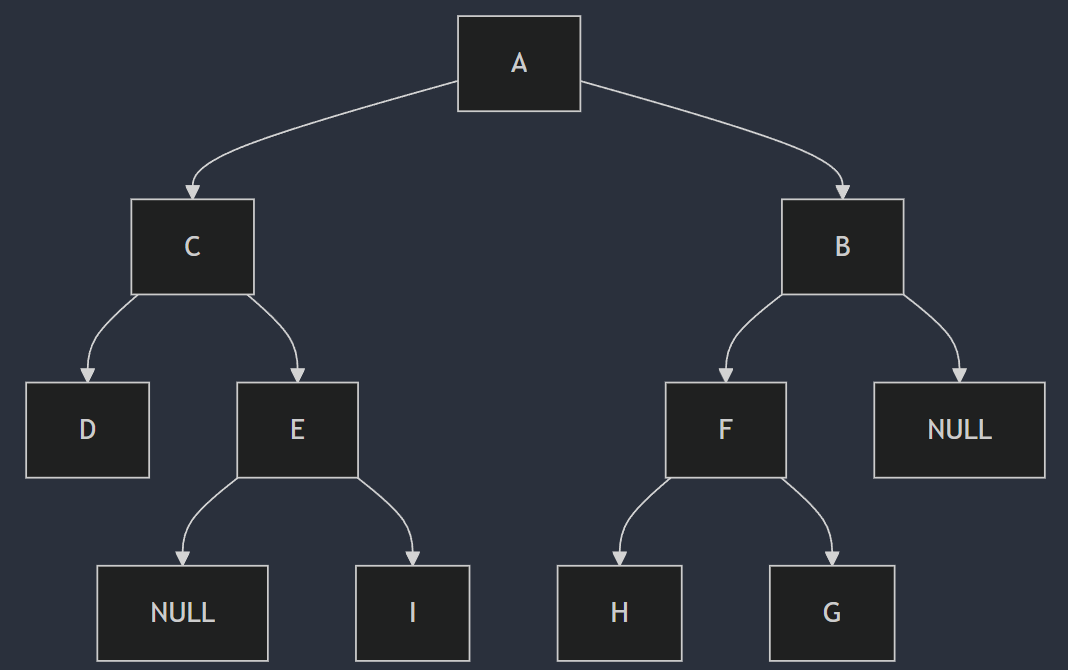
\includegraphics[width = 100mm]{binarytree.png}
  \end{center}
\end{figure}
次に、binarytree.cを以下のmakeコマンドを実行してコンパイルし、プログラムを実行する。
\begin{lstlisting}
  PS C:\Users\daiki\Desktop\DSA\kadai4> make
  gcc    -c -o binarytree.o binarytree.c
  gcc   binarytree.o main_binarytree.o   -o binarytree
  PS C:\Users\daiki\Desktop\DSA\kadai4> ./binarytree
  PRE: A C D E I B F H G 
  IN: D C E I A H F G B
  POST: D I E C H G F B A
  BFS: A C B D E F I H G
  TREE: A(C(D(null,null),E(null,I(null,null))),B(F(H(null,null),G(null,null)),null))
  height: 4
\end{lstlisting}
まず、create\_nodeで図で表されている二分木を作成した。
preorder、inorder、postorder、breadth\_first\_searchでそれぞれラベルを表示した。図と比較してみると正しく出力されていることがわかる。
displayの出力も図と比較すれば正しく表示されていることがわかる。
heightも図を見ると木の高さが4なので正しく出力されている。
最後にdelete\_treeで確保したメモリ領域を開放した。
これらの関数は\ref{subsubsec:実装コードおよびコードの説明1}で説明したように動作する。
以上より基本課題の要件をすべて満たすことを確認した。

\subsection{2分探索木の実装}
\subsubsection{実装の方針}
まず、2分探索木の機能として、rootを根とする二分探索木における最小値を
探索し、その値を返し、二分探索木画からの場合は-1を高さとして返すmin\_bst(Node *root)、
整数dがrootを根とする二分探索木二存在するか検査し、存在すればtrue、存在しなければfalseを
bool型で返すsearch\_bst(Node *root,int d)、rootを根とする二分探索木に整数dを追加し、二分探索木が
からの場合は、整数dの根を作成するinsert\_bst(Node **root,int d)、rootを根とする二分探索木から
整数dを削除するdelete\_bst(Node **root,int d)をbinarysearchtree.cに実装した。
また、main関数は別ファイルmain\_binarysearchtree.cに実装した。
\subsubsection{実装コードおよびコードの説明}\label{subsubsec:実装コードおよびコードの説明2}
プログラム\ref{code:two}に、binarysearchtree.cの主要部を示す。\\ \indent
int min\_bst(Node *root)関数は、葉を除く任意の節点nに対して、その節点のデータは左部分木内の任意のデータより
大きく、右部分木内の任意のデータより小さいという条件から最左端ノードのデータが最小値を取るという性質を用いて、
左の子ノードがNULL出ない限り左の子ノードに移動し続け、NULLになったときそのノードは最左端ノードなので
そのノードのデータを返す。
bool search\_bst(Node *root,int d)関数は、上述した二分探索木の性質を利用して、探索対象の整数dよりpの
データが大きい場合は左部分木に、小さい場合は右部分木に移動し、値が等しい場合は探索対象が見つかったのでtrueを返す。
探索しても見つからなかった場合はfalseを返す。
void insert\_bst(Node **root,int d)関数は、関数内でNode型ポインタrootが保持するアドレスを書き換えるため、
Node型のポインタのポインタを第一引数にセットしている。ルートノードが空であれば、新しいノードを作成し、木のルートとして
設定する。ノードの作成には\ref{subsec:2分木の実装}で説明したcreate\_nodeを用いた。木がから出ない場合、ルートノードから始めて、
次の手順で挿入位置を探索する。pポインタで現在のノードを追跡、挿入する値dを現在のノードの値と比較、dと等しい場合は
挿入せず終了。dより大きい場合は左部分木を探索。もし左の子ノードが空なら新しいノードを挿入。dより小さい場合は右部分木を
探索。もし右の子ノードが空なら新しいノードを挿入。
void delete\_bst(Node **root,int d)関数は、insert\_bstと同様に第一引数にNode型ポインタのポインタを持つ。
ルートノードが空の場合、何もせずに終了。そうでなければルートノードから順にノードを探索する。削除対象のノードをp、
その親ノードをqに記録する。pのデータがdより大きい場合は左部分木、小さい場合は右部分木に移動する。ノードが見つからない場合は
関数を終了する。pの子ノードの数に応じて次のケースを処理する。case1:子を持たないノードの場合、親ノードqから対象ノードpを
取り外し、pを開放する。もしpが根ノードの場合、ルートノードを空にする。case2:1つの子を持つノード場合、pの子ノードを親ノード
qに接続し、ノードpを開放する。もしpが親ノードの場合、ルートノードを子ノードに更新する。case3:2つの子を持つノードの場合、
右部分木の最小値ノードsを探索し、削除対象ノードpの値をsの値で置き換える。最小値ノードsは子を持たないか、右部分木を持つため、
その後sを削除する。

\begin{lstlisting}[caption=binarysearchtree.cの主要部, label=code:two, language=C,captionpos = b]
int min_bst(Node *root){
    if(root == NULL)return -1;
    Node *p = root;
    while(p->left != NULL)p = p->left;
    return p->value;
}

bool search_bst(Node *root, int d){
    Node *p = root;
    while(p != NULL){
        if(p->value == d){
            return true;
        } else if (p->value > d){
            p = p->left;
        } else {
            p = p->right;
        }
    }
    return false;
}

void insert_bst(Node **root, int d){
    if(*root == NULL){
        *root = create_node(d, NULL, NULL);
        return;
    }
    Node *p = *root;
    while(1){
        if(p->value == d)return;
        if(p->value > d){
            if(p->left == NULL){
                p->left = create_node(d,NULL,NULL);
                return;
            } else {
                p = p->left;
            }
        } else {
            if(p->right == NULL) {
                p->right = create_node(d,NULL,NULL);
                return;
            } else {
                p = p->right;
            }
        }
    }
}

void delete_bst(Node **root, int d) {
    if (*root == NULL) return;

    Node *p = *root;
    Node *q = NULL;

    while (p != NULL && p->value != d) {
        q = p;
        if (d < p->value) {
            p = p->left;
        } else {
            p = p->right;
        }
    }

    if (p == NULL) return;

//case1
    if (p->left == NULL && p->right == NULL) {
        if (q == NULL) {
            *root = NULL;
        } else if (q->left == p) {
            q->left = NULL;
        } else {
            q->right = NULL;
        }
        free(p);

//case2
    } else if (p->left == NULL || p->right == NULL) {
        Node *child = (p->left != NULL) ? p->left : p->right;

        if (q == NULL) {
            *root = child;
        } else if (q->left == p) {
            q->left = child;
        } else {
            q->right = child;
        }
        free(p);

//case3
    } else {
        Node *s = p->right;
        Node *sp = p;

        while (s->left != NULL) {
            sp = s;
            s = s->left;
        }

        p->value = s->value;

        if (sp->left == s) {
            sp->left = s->right;
        } else {
            sp->right = s->right;
        }
        free(s);
    }
}
\end{lstlisting}
\subsubsection{実行結果}\label{subsubsec:実行結果2}
まず、main\_binarysearchtree.cの主要部を以下に示す。
\begin{lstlisting}
int main(void) {
    // Build a binary search tree
    Node *root = NULL;
    insert_bst(&root, 10);
    insert_bst(&root, 15);
    insert_bst(&root, 18);
    insert_bst(&root, 6);
    insert_bst(&root, 12);
    insert_bst(&root,  20);
    insert_bst(&root,  9);

    inorder(root);
    display(root);

    printf("search_bst 10: %d\n", search_bst(root, 10));
    printf("search_bst 12: %d\n", search_bst(root, 12));
    printf("search_bst 15: %d\n", search_bst(root, 15));
    printf("search_bst 7: %d\n", search_bst(root, 7));
    printf("min_bst: %d\n", min_bst(root));

    delete_bst(&root, 15);

    inorder(root);
    display(root);

    delete_bst(&root, 10);

    inorder(root);
    display(root);

    delete_tree(root);

    root = NULL;
    printf("search_bst 10: %d\n", search_bst(root, 10));

    return EXIT_SUCCESS;
}   
\end{lstlisting}
\newpage
今回は次の図で表す二分木に対して、実装した関数が正しく動作することを確認する。
\begin{figure}[htbp]
  \begin{center}
      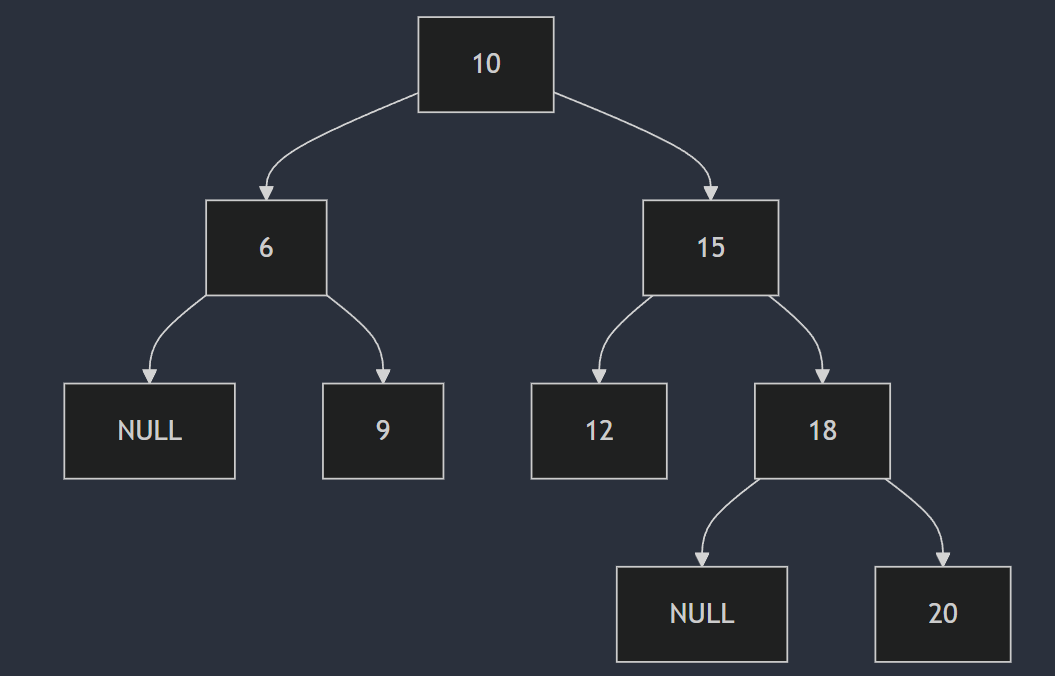
\includegraphics[width = 100mm]{binarysearchtree1.png}
  \end{center}
\end{figure}
次に、binarysearchtree.cを以下のmakeコマンドを実行してコンパイルするためにMakefileに以下の行を追加した。
\begin{lstlisting}
  CC:=gcc
  binarytree: binarytree.o main_binarytree.o
  binarysearchtree: binarysearchtree.o main_binarysearchtree.o #add
\end{lstlisting}
makeコマンドでコンパイルし、プログラムを実行した結果は以下のようになった。
\begin{lstlisting}
  PS C:\Users\daiki\Desktop\DSA\kadai4> ./binarysearchtree   
  IN: 6 9 10 12 15 18 20 
  TREE: 10(6(null,9(null,null)),15(12(null,null),18(null,20(null,null))))
  search_bst 10: 1
  search_bst 12: 1
  search_bst 15: 1
  search_bst 7: 0
  min_bst: 6
  6 9 10 12 18 20
  TREE: 10(6(null,9(null,null)),18(12(null,null),20(null,null)))
  6 9 12 18 20
  TREE: 12(6(null,9(null,null)),18(null,20(null,null)))
  search_bst 10: 0
\end{lstlisting}
まず、insert\_bstで値10,15,18,6,12,20,9をこの順で挿入した結果は図のような二分探索木になった。
inorderで表示した結果も値の小さい順に表示されているので正しく挿入できていることが確認できる。
次に10,12,15,7をsearch\_bstで探索した結果を見ると、10は根、12は葉、15は根以外の非終端節点、
7は二分探索木に無いデータとなっており、全て正しく探索できていることが確認できる。\\
delete\_bstで15を削除した際の二分探索木をdisplayで表示した結果が正しいかを図を用いて確認する。
15は2つの子を持ち、右部分木内で最も小さい値は18なので、18の部分木は移動せず、15の位置に18が移動するはずである。
以下にその図を示す。
\begin{figure}[htbp]
  \begin{center}
      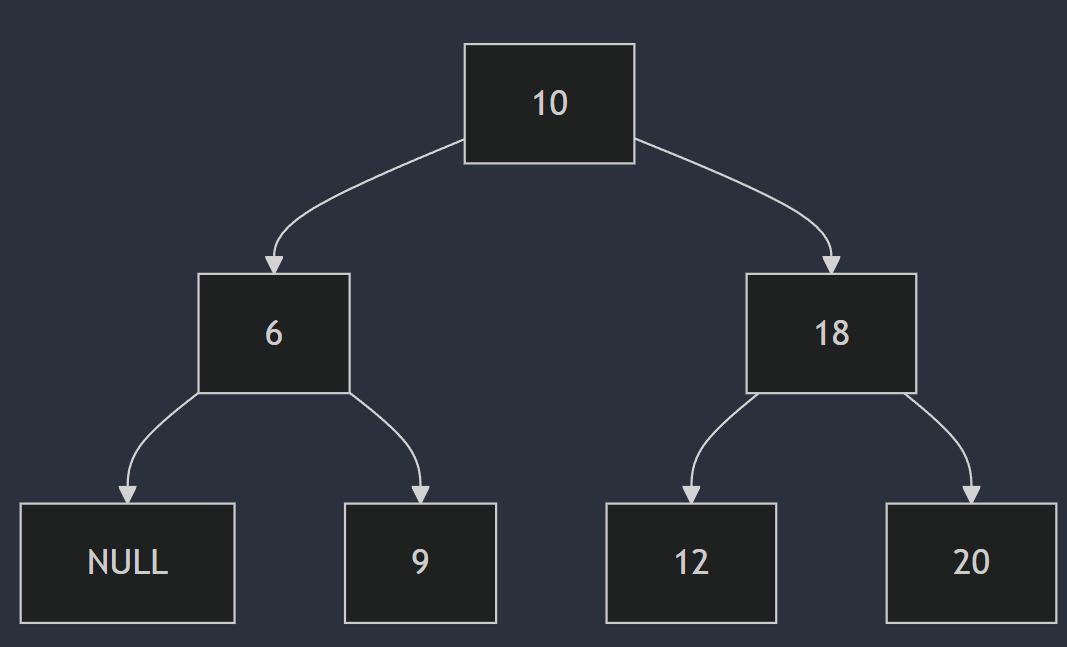
\includegraphics[width = 100mm]{binarysearchtree2.png}
  \end{center}
\end{figure}
\ref{subsubsec:実装コードおよびコードの説明2}で説明したように動作するならば図のような木構造になるはずである。
displayでの表示結果と見比べると木構造が一致していることがわかるので正しく削除できていることを確認した。
さらに、根である10を削除する場合、子を2つ持つので、右の部分木内で最小の値である12が先程述べた処理同様に10の位置に
移動する。displayの表示結果を見ても12が根の位置に移動しているので正しく実装されていることがわかる。
また、delete\_treeで二分探索木を削除した後に空の木を作成し、search\_bstで探索した結果、
0が表示されているので正しき探索できている。\\
以上の処理は\ref{subsubsec:実装コードおよびコードの説明2}で説明したとおりに動作する。よってこの課題の

\end{document}